\iffalse
\def\mytitle{OPTIMIZATION}
\def\myauthor{VUNNAVA SRAVANI}
\def\contact{sravani21vunnava@gmail.com}
\def\mymodule{Future Wireless Communication (FWC)}
\documentclass[10pt, a4paper]{article}
\usepackage[a4paper,outer=1.5cm,inner=1.5cm,top=1.75cm,bottom=1.5cm]{geometry}
\twocolumn
\usepackage{setspace}
\usepackage{graphicx}
\graphicspath{{./images/}}
\usepackage[colorlinks,linkcolor={black},citecolor={blue!80!black},urlcolor={blue!80!black}]{hyperref}
\usepackage[parfill]{parskip}
\usepackage{lmodern}
\usepackage{tikz}
	\usepackage{physics}
%\documentclass[tikz, border=2mm]{standalone}
\usepackage{karnaugh-map}
\usepackage{tabularx}
\usetikzlibrary{calc}
\usepackage{amsmath}
\usepackage{amssymb}
\renewcommand*\familydefault{\sfdefault}
\usepackage{watermark}
\usepackage{lipsum}
\usepackage{xcolor}
\usepackage{listings}
\usepackage{float}
\usepackage{titlesec}
\providecommand{\mtx}[1]{\mathbf{#1}}
\titlespacing{\subsection}{1pt}{\parskip}{3pt}
\titlespacing{\subsubsection}{0pt}{\parskip}{-\parskip}
\titlespacing{\paragraph}{0pt}{\parskip}{\parskip}
\newcommand{\figuremacro}[5]{//
    \begin{figure}[#1]
        \centering
        \includegraphics[width=#5\columnwidth]{#2}
        \caption[#3]{\textbf{#3}#4}
        \label{fig:#2}
    \end{figure}
}
\newcommand{\myvec}[1]{\ensuremath{\begin{pmatrix}#1\end{pmatrix}}}
\let\vec\mathbf
\lstset{
frame=single, 
breaklines=true,
columns=fullflexible
}

\title{\mytitle}
\author{\myauthor\hspace{1em}\\\contact\\FWC22012\hspace{6.5em}IITH\hspace{0.5em}\mymodule\hspace{6em}ASSIGN-8}
\date{}
\begin{document}
	\maketitle
	\tableofcontents

\section{Construction}
\includegraphics[scale=0.5]{fig.pdf}

\section{Problem}
\fi
Maximize 
\begin{align}
Z = x+y 
\end{align}
subject to
\begin{align}
 x - y &\le -1
	\\
	-x+y&\le0 
	\\
	x,y &\ge 0
\end{align}
\solution 
	\begin{figure}[!ht]
		\centering
		\includegraphics[width=\columnwidth]{12/12/1/10/figs/fig.pdf}
		\caption{}
		\label{fig:12/12/1/10}
  	\end{figure}
	From Fig. 
		\ref{fig:12/12/1/10},
		the given problem has no optimal solution.  This is verified from cvxpy by considering the following optimization problem.
	\iffalse
\section{Solution}
Consider,
\begin{tabular}{|c|c|}
	\hline
	\textbf{Parameter}&\textbf{Value}\\
	\hline
	$\vec{c}$ & $\myvec{1\\1}$ \\
	\hline
	$\vec{x}$ & $\myvec{x\\y}$ \\
	\hline
	$\vec{p}$ & $\myvec{1&-1 \\ -1&0 \\ 0&-1 \\ -1&0}$ \\
	\hline
\end{tabular}\\

Objective function:
Constraints:
\begin{align}
x - y\le -1
\end{align}
\begin{align}
-x + y \le 0
\end{align}
\begin{align}
-x \le 0
\end{align}
\begin{align}
-y \le 0
\end{align}
writing all the constraints in matrix form:
\begin{align}
\vec{p^T}\vec{x} \preceq \vec{q}
\end{align}
\fi
\begin{align}
	z = \max_{x}\myvec{1 & 1}\vec{x}
	\\
	s.t. \quad
\myvec{1&-1 \\ -1&0 \\ 0&-1 \\ -1&0}x \preceq \myvec{-1 \\ 0 \\ 0 \\ 0 }
\end{align}
\iffalse
By providing the objective function and constraints to cvxpy, we get the optimal solution for z
\\
\textbf{cvxpy code}

from cvxpy code,\\
There is no feasible region between,\\
Hence there is no maximum value for z.

\end{document}
\fi
